% ======================================================================
% Inicio del preámbulo 
% ======================================================================

\documentclass[12pt,letterpaper]{article}
\usepackage[left=2cm, top=2.5cm, bottom=2.5cm, right=2cm]{geometry}
\usepackage[spanish]{babel}
\selectlanguage{spanish}

\usepackage[utf8]{inputenc} % Reconocimiento de tildes y otros caracteres
\usepackage{graphicx}
\usepackage{setspace}
\usepackage[scaled]{helvet}
\renewcommand\familydefault{\sfdefault}
\usepackage[justification=centering]{caption}
\usepackage[labelfont=bf]{caption}
\usepackage {amsmath, amssymb, multicol, cancel} % cargar librerías para fórmulas símbolos y otras cosas
\usepackage{placeins}
\usepackage{float} % forzar la figura en la subsección que le corresponde
\usepackage{pdfpages}

\addto\captionsspanish{\renewcommand{\tablename}{Tabla}} % Cambiar nombre a tablas

\usepackage{hyperref} % permite agregar links
\hypersetup{
    colorlinks=true,
    linkcolor=black,
    urlcolor=blue,
    citecolor=black,
    } % características de los links

\def \imgwidth {150mm} % ancho de las figuras

% ======================================================================
% Fin del preámbulo 
% ======================================================================

\begin{document}

\begin{titlepage}
\begin{center}
\textbf{UNIVERSIDAD DE COSTA RICA}\\ 
\vspace{6mm}
\textbf{ESCUELA DE INGENIERÍA ELÉCTRICA}\\
\vspace{3cm}
\textbf{IE0624}\\
\textbf{Laboratorio de Microcontroladores}\\
\vspace{3cm}
\textbf{Laboratorio III}\\
\vspace{0.5cm}
Arduino: PID, GPIO, ADC y comunicaciones\\
\vspace{3cm}
Estudiantes:\\
Kendall Saborio Picado - B87103\\
Alexander Rojas Brenes - B86869\\
\vspace{1.5cm}
Profesor:\\
Ing. Marco Villalta Fallas
\vfill
Fecha de entrega: 08/05/2021
\end{center}
\end{titlepage}

\tableofcontents

\newpage
\section{INTRODUCCIÓN}
 Este trabajo aborda el desarrollo de un sistema de monitoreo de pendientes, diseñado para detectar peligros potenciales en una etapa temprana y proporcionar alertas y predicciones tempranas. El objetivo principal de este sistema es permitir a las autoridades pertinentes tomar medidas adecuadas antes de que ocurra un incidente. El sistema se construyó utilizando una placa STM32F429 Discovery kit y la biblioteca libopencm3. Para lograr el monitoreo de pendientes, se leen los ejes del giroscopio (X, Y, Z) y la temperatura. Se implementó un mecanismo de alerta mediante un LED parpadeante que se activa cuando se detecta una deformación angular mayor a 5 grados en cualquier eje. Además, se envía una notificación de advertencia al dashboard de ThingsBoard, una plataforma de IoT de código abierto basada en Java. El sistema también monitorea el nivel de la batería, cuyo rango operativo es de [0,9]V. Si el nivel de la batería se acerca al límite mínimo de operación del microcontrolador (7V), se enciende un LED de alarma parpadeante y se envía una notificación de batería baja al dashboard de ThingsBoard. Para ello, se utiliza una batería de 9V y un circuito que condiciona el nivel de voltaje dentro del rango de operación del microcontrolador. En la pantalla LCD del sistema se despliegan el nivel de batería, la temperatura, los valores de los ejes X, Y, Z y el estado de la comunicación serial/USB. Se utiliza un botón de la placa para habilitar o deshabilitar las comunicaciones por USART/USB. Además, se desarrolló un script en Python que permite leer y escribir al puerto serial/USB, enviando la información del giroscopio, temperatura y nivel de batería al dashboard de ThingsBoard.
 Para consultar el trabajo realizado, puede consultarse el siguiente repositorio de trabajo, en la rama llamada ``Lab4'': \url{https://github.com/SaboEIE/IE-0624_IS_2024_B87103.git}. El código principal en C \texttt{lab4.c}, los archivos necesarios extraídos de la librería, el archivo en python \texttt{iot.py} y el Makefile puede consultarse en la ruta \path{Laboratorio_04/src}. 
 

\newpage
\section{NOTA TEÓRICA}

Antes de iniciar con el uso y manipulación del lenguaje de programación C para la creación de los algoritmos objetivo del presente laboratorio, es necesario tener a mano una serie de conceptos importantes, los cuales se explican a continuación: 

\subsection{Microcontrolador STM32F429}
Tal como se detalla en la hoja del fabricante \cite{ST}, el STM32F429 es un microcontrolador de 32 bits desarrollado por STMicroelectronics, perteneciente a la familia STM32, que se basa en el núcleo ARM Cortex-M4 que opera a una frecuencia de hasta 180 MHz.. Este microcontrolador es conocido por su alto rendimiento, amplia gama de periféricos y altas capacidades que lo hacen ideal para aplicaciones complejas en una variedad de campos, como la electrónica de consumo, la automatización industrial y las telecomunicaciones.

Incluye instrucciones específicas para el procesamiento digital de señales (DSP), que son particularmente útiles para aplicaciones que requieren cálculos matemáticos intensivos, una memoria flash con capacidad de 2 MB y una SRAM de 256Kb. Asimismo, cuenta con hasta 168 GPIO programables, 17 timers (6 timers generales de 16 bits y 4 timers generales de 32 bits). Posee un controlador TFT-LCD que permite la conexión directa a pantallas TFT, facilitando el desarrollo de interfaces gráficas. Soporte para interfaces de cámaras digitales, útil en aplicaciones de visión artificial. Incluye varios interfaces como USB OTG (On-The-Go), Ethernet, CAN (Controller Area Network), y varios puertos UART, SPI, I$^2$C, entre otros. Este microcontrolador dispone de 3 ADCs independientes de 12 bits, puede manejar hasta 24 canales, permitiendo la adquisición de señales de múltiples fuentes analógicas. 

En la Figura \ref{fig:ST_pins} puede observarse la distribución de pines del microcontrolador y sus respectivas funciones:  

\begin{figure}[H]
\centering
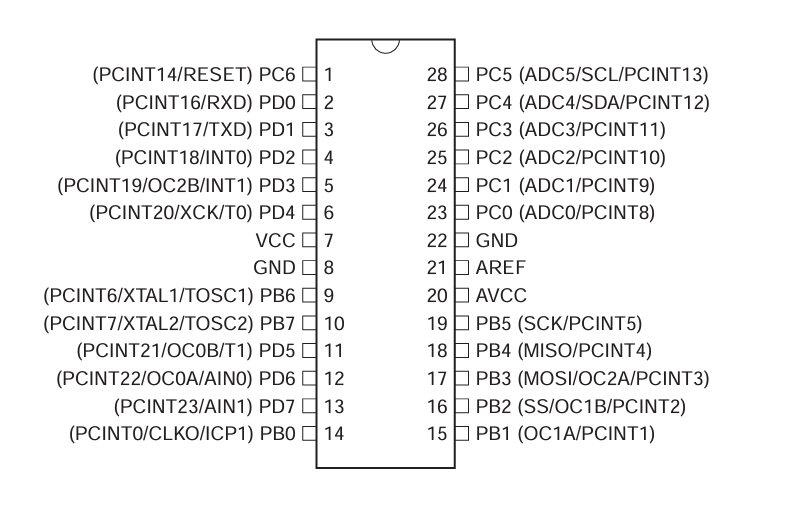
\includegraphics[scale=0.5]{./Figuras/Nota_teorica/PINES}
\caption{Diagrama de pines y sus respectivas funciones. (Fuente: Imagen tomada de \cite{ST})}
\label{fig:ST_pins}
\end{figure}

Para más información general del dispositivo, observar el Anexo \ref{an:01_GEN}. Por otro lado, en la Figura \ref{fig:DBLO} puede consultarse el diagrama de bloques del microcontrolador en el cual puede consultarse a alto nivel la conexión interna de este (no incluye el CPU):

\begin{figure}[H]
\centering
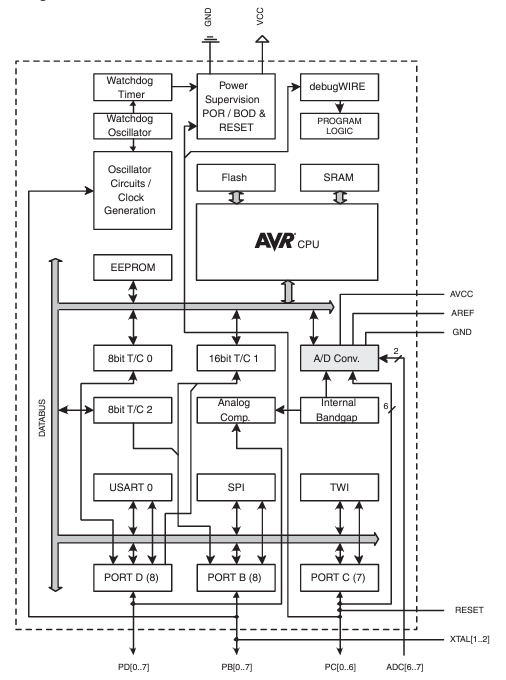
\includegraphics[width=160mm]{./Figuras/Nota_teorica/Bloques}
\caption{Diagrama de bloques del STM32F429. (Fuente: Imagen tomada de \cite{ST})}
\label{fig:DBLO}
\end{figure}



\subsubsection{Registros de importancia}
Según la hoja del fabricante \cite{ST}, el mapa de memoria del STM32F427xx y STM32F429xx está dividido en varias regiones, cada una asignada a diferentes tipos de periféricos y funcionalidades. A continuación, se muestran los rangos de direcciones de registros de importancia:

\begin{figure}[H]
\centering
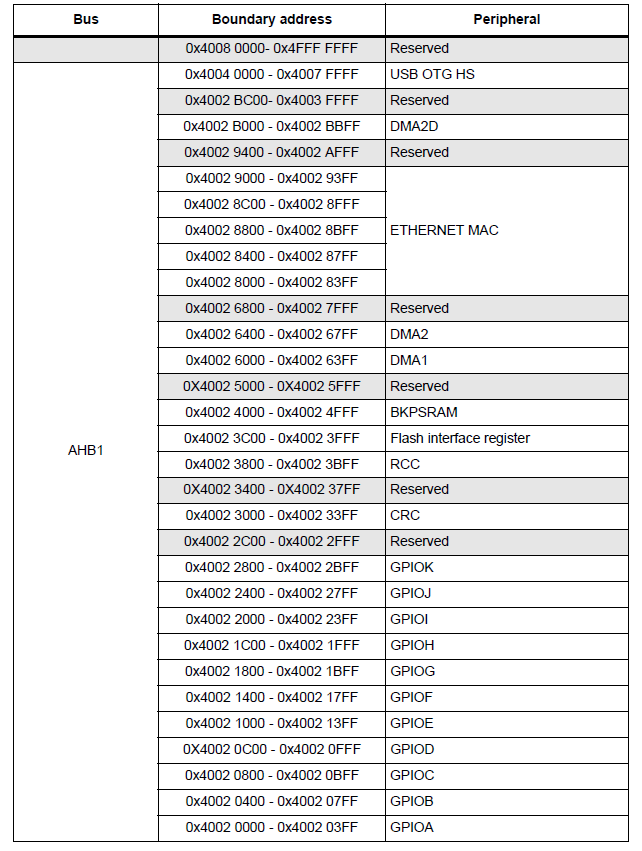
\includegraphics[scale=0.8]{./Figuras/Nota_teorica/REGS1}
\caption{Rangos direcciones de registros. (Fuente: Imagen tomada de \cite{ST})}
\label{fig:REGS1}
\end{figure}


\begin{figure}[H]
\centering
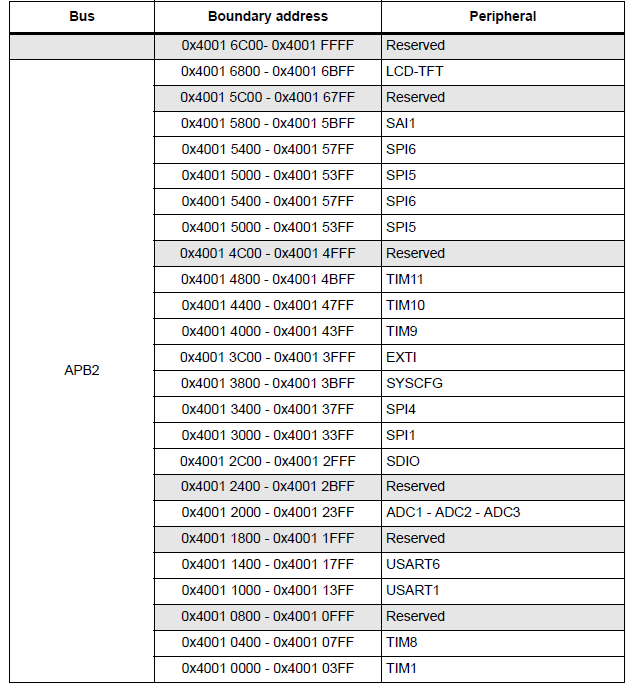
\includegraphics[scale=0.8]{./Figuras/Nota_teorica/REGS2}
\caption{Rangos direcciones de registros. (Fuente: Imagen tomada de \cite{ST})}
\label{fig:REGS2}
\end{figure}

\begin{figure}[H]
\centering
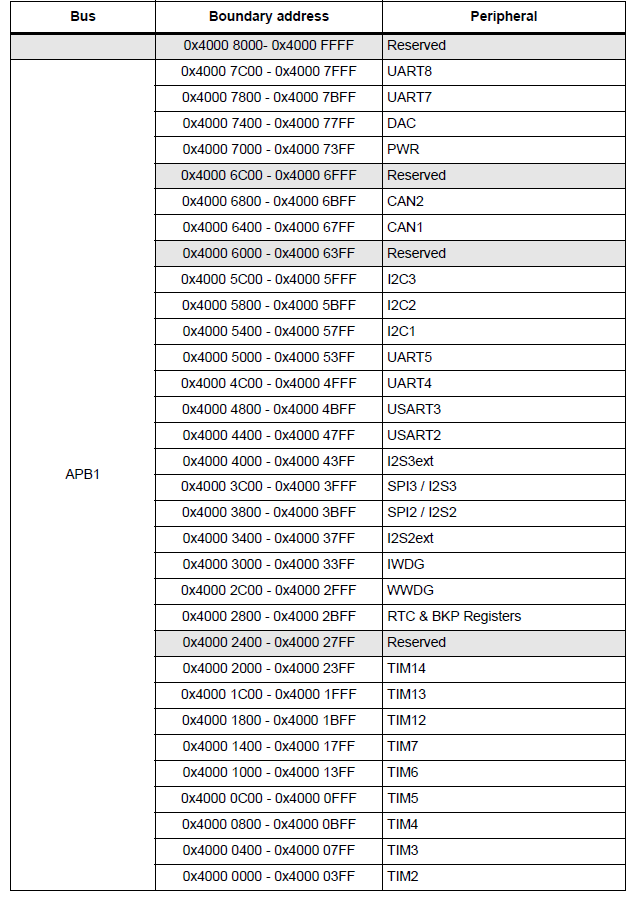
\includegraphics[scale=0.8]{./Figuras/Nota_teorica/REGS3}
\caption{Rangos direcciones de registros. (Fuente: Imagen tomada de \cite{ST})}
\label{fig:REGS3}
\end{figure}

Es importante mencionar que el caso de este microcontrolador, se puede utilizar ciertas librerías como LibOpenCM3 que proporcionan una capa de abstracción más alta sobre el hardware, lo que significa que facilita manipular los registros del microcontrolador.

\subsubsection{Características eléctricas}
A continuación se muestra las especificaciones eléctricas del STM32F429:

%%%%%%%%%%%%%%%%%%
\begin{figure}[H]
\centering
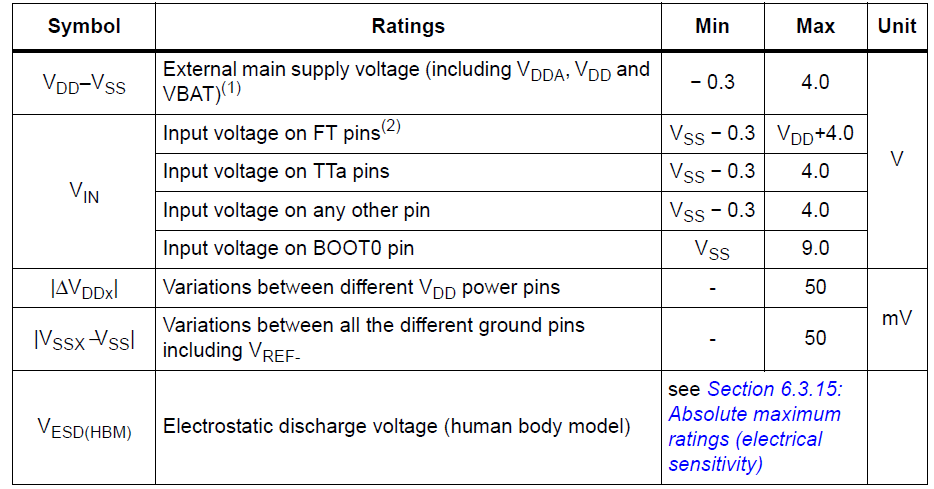
\includegraphics[scale=0.6]{./Figuras/Nota_teorica/ELEC1}
\caption{Características de tensión. (Fuente: Imagen tomada de \cite{ST})}
\label{fig:ELEC1}
\end{figure}

%%%%%%%%%%%%%%%%%%
\begin{figure}[H]
\centering
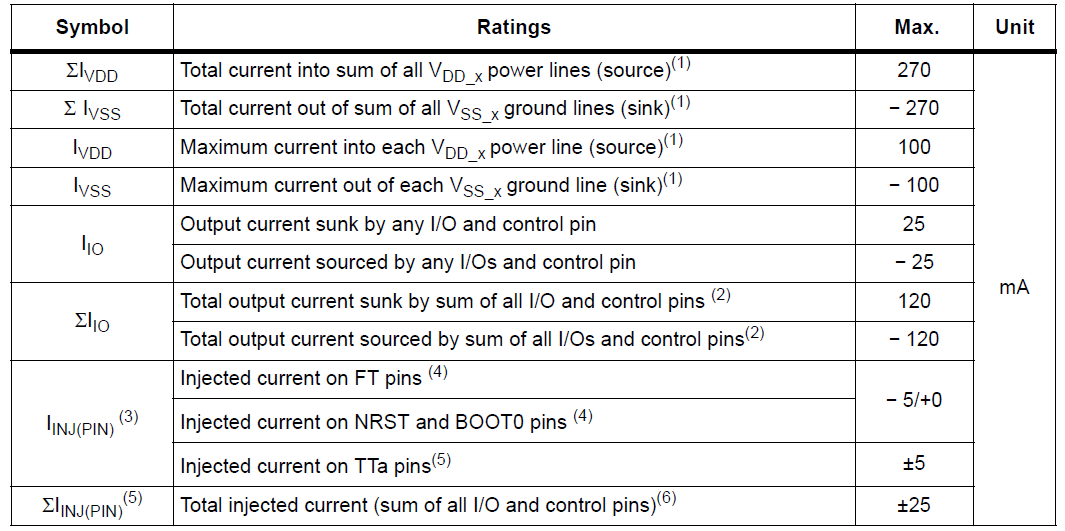
\includegraphics[scale=0.6]{./Figuras/Nota_teorica/ELEC2}
\caption{Características de corriente. (Fuente: Imagen tomada de \cite{ST})}
\label{fig:ELEC2}
\end{figure}

\subsubsection{Sensor L3GD20}
El sensor MEMS L3GD20 es un giroscopio digital de 3 ejes fabricado por STMicroelectronics, diseñado para medir la velocidad angular en aplicaciones de movimiento y orientación. Este sensor puede medir la velocidad angular alrededor de tres ejes ortogonales (X, Y, Z), con un rango de medición seleccionable entre ±250 dps, ±500 dps, y ±2000 dps. Posee una alta resolución de 16 bits para cada eje y una sensibilidad ajustable según el rango de medición seleccionado, lo que permite obtener datos precisos en diferentes aplicaciones. El L3GD20 se comunica con los microcontroladores a través de interfaces SPI (Serial Peripheral Interface) y I2C (Inter-Integrated Circuit), con una tasa de salida de datos (ODR) seleccionable de 95 Hz a 760 Hz. \cite{L3} 

El L3GD20 también incluye funcionalidades avanzadas, como la integración de filtros paso bajo y paso alto programables, detección de interrupciones programables para eventos específicos (como caída libre y movimiento), y una función de auto-prueba para verificar su correcto funcionamiento. Funciona con un voltaje de operación de 2.4V a 3.6V y en un rango de temperatura de -40°C a +85°C, haciéndolo adecuado para diversas aplicaciones ambientales \cite{L3}.

El sensor puede integrarse con el microcontrolador STM32F429 utilizando sus interfaces SPI o I2C. Esto implica conectar los pines SPI/I2C del L3GD20 a los pines apropiados del STM32F429 y asegurar una correcta alimentación del sensor. Luego, se configura el STM32F429 para comunicarse con el L3GD20 utilizando las bibliotecas HAL (Hardware Abstraction Layer) o LL (Low Layer) proporcionadas por STMicroelectronics \cite{L3}. A continuación algunos de los registros esenciales para su configuración y funcionamiento:

\begin{itemize}
    \item \textbf{CTRL\_REG1} (0x20): Controla el encendido del sensor y la configuración básica de la tasa de salida de datos y los filtros.
    \begin{itemize}
        \item Bits 7-6: Selección de la tasa de salida de datos (ODR).
        \item Bits 5-4: Selección del ancho de banda del filtro de paso bajo.
        \item Bit 3: Control de encendido del giroscopio.
        \item Bits 2-0: Habilitación de los ejes X, Y y Z.
    \end{itemize}

    \item \textbf{CTRL\_REG2} (0x21): Configuración del filtro de paso alto.
    \begin{itemize}
        \item Bits 5-4: Modo de filtro de paso alto.
        \item Bits 3-0: Frecuencia de corte del filtro de paso alto.
    \end{itemize}

    \item \textbf{CTRL\_REG4} (0x23): Configuración del rango de escala y del auto-prueba.
    \begin{itemize}
        \item Bits 5-4: Selección del rango de escala (±250 dps, ±500 dps, ±2000 dps).
        \item Bit 3: Control del modo de auto-prueba.
        \item Otros bits para configuraciones adicionales.
    \end{itemize}

    \item \textbf{OUT\_TEMP} (0x26): Registro de salida de la temperatura, proporciona datos de temperatura.

    \item \textbf{OUT\_X\_L} (0x28) y \textbf{OUT\_X\_H} (0x29) : Registros de datos de salida del eje X (bajo y alto).

    \item \textbf{OUT\_Y\_L} (0x2A) y \textbf{OUT\_Y\_H} (0x2B) : Registros de datos de salida del eje Y (bajo y alto).

    \item \textbf{OUT\_Z\_L} (0x2C) y \textbf{OUT\_Z\_H} (0x2D) : Registros de datos de salida del eje Z (bajo y alto).
\end{itemize}


\subsubsection{Pantalla y gráficos}
La pantalla TFT-LCD integrada en los kits de desarrollo típicos del STM32F429, suele tener un tamaño de 2.4 a 2.8 pulgadas con una resolución de 240x320 píxeles (QVGA). La pantalla utiliza una interfaz RGB paralela de 16/18/24 bits para la transmisión de datos, lo que permite una rápida actualización de la imagen. Esta pantalla utiliza el controlador gráfico ILI9341 y un controlador táctil XPT2046 para la detección de toques. A nivel de comunicación, esta pantalla ofrece interfaces I2C y SPI, y en el contexto de la placa STM32F429 Discovery Kit, se comunica mediante la interfaz SPI5. Algunos otras características indicadas en la hoja del fabricante \cite{ST} son:

\begin{itemize}
    \item 2 capas de pantalla con FIFO dedicado (64x32 bits)
    \item Tabla de búsqueda de colores (CLUT) de hasta 256 colores (256x24 bits) por capa
    \item Hasta 8 formatos de color de entrada seleccionables por capa
    \item Mezcla flexible entre dos capas usando valor alfa (por píxel o constante)
    \item Parámetros programables flexibles para cada capa
    \item Hasta 4 eventos de interrupción programables
\end{itemize}


\subsection{Librerías de importancia}

A continuación se detallan las librerías más importantes que fueron utilizadas en el laboratorio: 

\subsubsection{LibOpenCM3}

LibOpenCM3 es una biblioteca diseñada para ser utilizada con microcontroladores ARM Cortex-M de diferentes fabricantes, como STMicroelectronics, NXP, Texas Instruments, y otros. Ofrece una API coherente y fácil de usar para manejar los periféricos comunes de estos microcontroladores, lo que simplifica el desarrollo de aplicaciones embebidas. LibOpenCM3 soporta una amplia gama de microcontroladores de varios fabricantes, incluyendo STM32 (de STMicroelectronics), LPC (de NXP), EFM32 (de Silicon Labs), y otros. Compatible con diversas herramientas de compilación y entornos de desarrollo, como GCC (GNU Compiler Collection), y puede integrarse con IDEs populares como Eclipse, Keil, y otros \cite{libopencm3}. 

\subsection{IOT: Internet of things}
El Internet de las cosas (IoT, por sus siglas en inglés) se refiere a una red abierta y completa de objetos inteligentes que tienen la capacidad de autoorganizarse, compartir información, datos y recursos, reaccionando y actuando ante situaciones y cambios en el entorno. Es un concepto que ha evolucionado desde la idea de que la primera versión de Internet trataba sobre datos creados por personas, mientras que la siguiente versión se trata de datos creados por cosas \cite{madakam2015internet}. 

\subsection{Diseño del circuito de alimentación sistema de monitoreo de pendiente} \label{sec:cir1}

Según se indica en el enunciado, el presente laboratorio tiene como objetivo construir un sistema encargado de monitorear los cambios en la pendiente de un terreno. Al existir la necesidad de que este circuito se encuentre en un lugar específico, es necesario que se autónomo respecto a la energía que consume. Por lo anterior, es necesario que el microcontrolador sea conectado a una batería de 9 V y que la tensión restante también sea reportada para evitar que el sistema se quede sin energía. Sin embargo, existe un problema y es que la tensión máxima permitida por el microcontrolador según su hoja del fabricante \cite{ST} es de 5 V, por lo que será necesario aplicar una división de tensión utilizando resistores.

Un divisor de voltaje es un simple circuito de resistores en serie que proporciona una fracción específica del voltaje de entrada como voltaje de salida. La relación entre el voltaje de entrada y salida se define por los valores de dos resistores, tal como se explica en \cite{DT}. En la Figura \ref{fig:DTD} puede observarse la disposición necesaria de los resistores:

\begin{figure}[H]
\centering
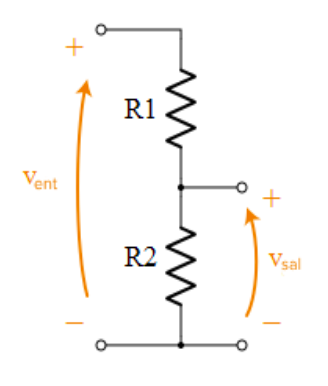
\includegraphics[width=55mm]{./Figuras/Nota_teorica/DTD}
\caption{Circuito de división de tensión.(Tomada de \cite{DT})}
\label{fig:DTD}
\end{figure}

Al pasar el diagrama anterior a expresiones matemáticas, de obtiene lo siguiente: 

\begin{equation}
    V_{sal} = V_{ent} \cdot \frac{R_{2}}{R_{1}+R_{2}} 
\end{equation}

Para el presente diseño, se seleccionó $R_{2} = 6.8 \; k\Omega$, además se sabe que la tensión de entrada es de 9 V y la tensión de salida debe ser de 5 V, por lo que sólo resta despejar el valor $R_1$: 

\begin{equation*}
    V_{sal} = V_{ent} \cdot \frac{R_{2}}{R_{1}+R_{2}} 
\end{equation*}

\begin{equation*}
    V_{sal} \cdot (R_{1}+R_{2}) = V_{ent} \cdot R_{2}
\end{equation*}

\begin{equation*}
    V_{sal} \cdot R_{1} + V_{sal} \cdot R_{2} = V_{ent} \cdot R_{2}
\end{equation*}

\begin{equation*}
    V_{sal} \cdot R_{1} = R_{2} \cdot (V_{ent} - V_{sal})
\end{equation*}

\begin{equation}
    R_{1} = R_{2} \cdot \frac{(V_{ent} - V_{sal})}{ V_{sal}}
\end{equation}

Sustituyendo los valores conocidos: 

\begin{equation}
    R_{1} = (6.8 \times 10^3) \cdot \frac{(9 - 5)}{5} = 5.44 \times 10^3 = 5.44 \; k\Omega
\end{equation}

Se selecciona un valor estándar, por lo que $R_1 = 5.6 \; k\Omega$. Lo anterior permitirá evitar sobrecargas de tensión en el microcontrolador y mantener su funcionamiento en condiciones controladas. 

\subsection{Lista de componentes y precios}

En la Tabla \ref{table:Equipo} pueden consultarse los componentes utilizados y sus precios, tomando como referencia los precios del sitio web de la tienda de componentes MicroJPM (\url{https://www.microjpm.com/}) y la página oficial de ST (\url{https://www.st.com/content/st_com/en.html}): 

\begin{table}[H]
\caption{Lista de componentes.}
\begin{center}
\begin{tabular}{c|c|c}
\hline
\textbf{Componente}&\textbf{Cantidad}&\textbf{Precio}\\
\hline
STM34F429I-DISC1 & 1 & \$29.30\\
Resistor de  k$\Omega$ & 1 & \$0,07\\
Resistor de  k$\Omega$ & 1 & \$0,07\\
Batería de 9 V $\Omega$ & 1 & \$5.64\\
\hline
Total & - & \$35.08\\
\end{tabular} \label{table:Equipo}
\end{center}
\end{table}

Según la Tabla \ref{table:Equipo}, para realizar este proyecto son necesario ₡18 073,50, según el valor del dólar al momento de escribir el presente informe. 

\newpage
\section{DESARROLLO Y ANÁLISIS DE RESULTADOS}

A continuación se muestran los métodos de desarrollo utilizados para resolver cada uno de los problemas planteados, así como la funciones utilizadas, el método de operación a partir de diagramas de flujo y los resultados obtenidos:

\subsection{Desarrollo de la solución}

A continuación podrá consultarse una descripción de alto nivel de cada una de las funciones implementadas para conseguir los objetivos del presente laboratorio: 

\subsubsection{Función \texttt{setup()}}
Esta función se encarga de inicializar todo lo necesario para que el proyecto funcione correctamente.Configura los pines de salida para los LEDs y de entrada para los dispositivos LCD y Serial, además inicia la comunicación con el LCD y configura el modo de operación del controlador PID en modo automático.

\subsubsection{Función \texttt{simPlanta()}}
Esta función se proporcionada por el enunciado. Simula el comportamiento térmico de un bloque de aluminio con calentamiento y enfriamiento pasivo, que vendría a tomar el comportamiento de la incubadora. Dentro de la función se calcula la temperatura del bloque de aluminio en función del tiempo, considerando la transferencia de calor desde un calentador y el enfriamiento por convección al ambiente. La función recibe como parámetro la cantidad de calor \texttt{Q} suministrado al bloque de aluminio (J/s). Esta función retorna la temperatura actual \texttt{T} del bloque de aluminio (°C).

\subsubsection{Función \texttt{LED\_control()}}
Esta función controla el encendido y apagado de los LEDs en base a la temperatura externa medida en la planta. La función recibe como parámetro \texttt{out\_temp} Temperatura de salida medida (en grados Celsius).
\subsubsection{Función \texttt{LCD\_control()}}
Esta función actualiza la pantalla LCD con las temperaturas operativa, de salida y la salida del controlador PID (Señal de control). La función recibe como parámetros \texttt{op\_temp} temperatura operativa actual (en grados Celsius), \texttt{PID} salida del controlador PID, \texttt{out\_temp} temperatura de salida actual de la planta (en grados Celsius).. 



\subsubsection{Función \texttt{serial\_com()}}
Función que imprime valores en el puerto serial. Esta función agrupa los valores de la temperatura de operación, la señal de control y la señal de salida de la planta, de forma que estos puedan ser captados y utilizados en futuro procesamiento. Cuenta con tres parámetros de tipo \texttt{double}: \texttt{op\_temp}, \texttt{PID} y \texttt{out\_temp}, los cuales representan la temperatura de referencia, la señal de control y la temperatura de salida de a planta.

\subsubsection{Función \texttt{loop()}}
\texttt{loop()} es la función principal del programa, realiza las siguientes operaciones en un ciclo continuo:
\begin{itemize}
    \item Lee el valor del potenciómetro.
    \item Mapea el valor leído a un rango de 20 a 80.
    \item Actualiza el valor de referencia del controlador PID (Setpoint).
    \item Calcula la salida del controlador PID.
    \item Convierte la salida en temperatura del controlador PID a watts.
    \item Simula el comportamiento térmico de la planta y obtiene la temperatura de salida.
    \item Controla los LEDs en función de la temperatura de salida.
    \item Actualiza la pantalla LCD si el pin de control está en estado alto.
    \item Inicia o detiene la comunicación serial si el pin de control está en estado alto.
\end{itemize}


\subsubsection{Diagrama de Flujo}
A continuación se muestra un diagrama de flujo del código en C utilizado para este laboratorio:

\begin{figure}[H]
    \centering
        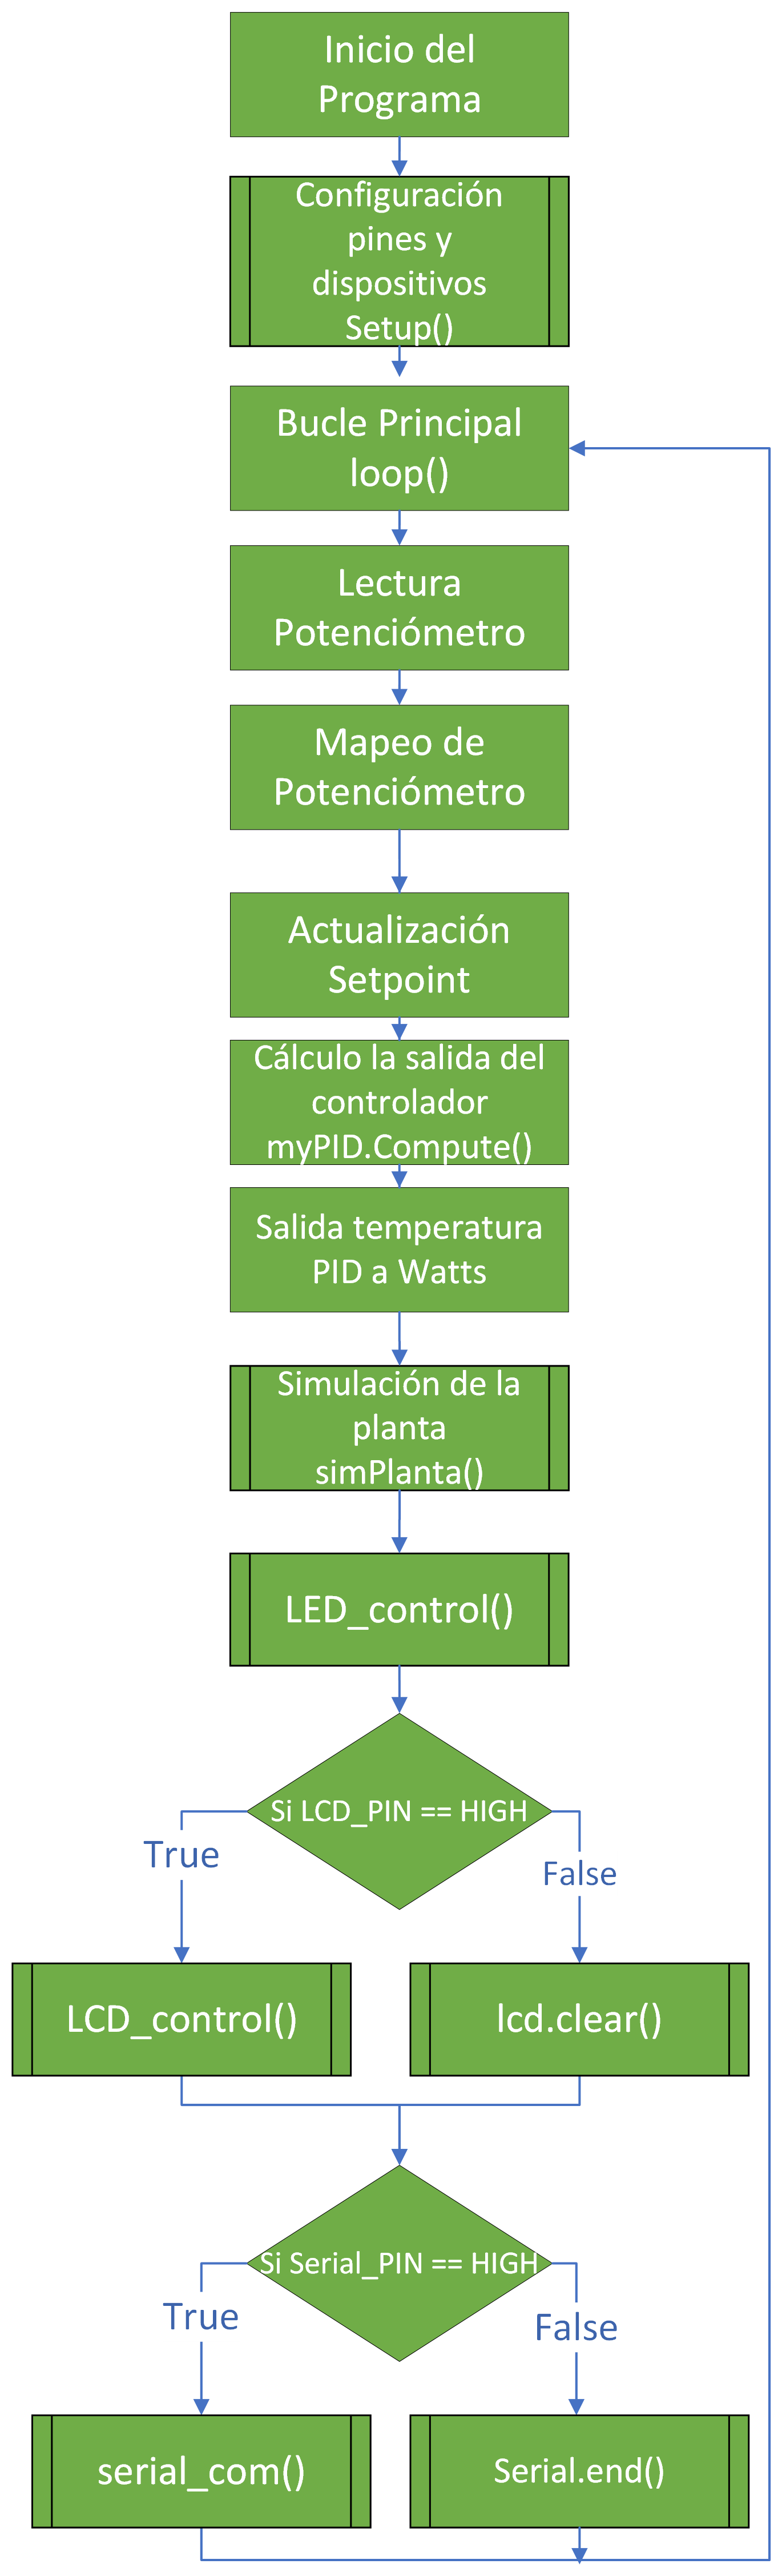
\includegraphics[scale = 0.58]{./Figuras/Desarrollo_Analisis/DF.png}
        \caption{Diagrama de flujo que describe el funcionamiento del sistema.}
    \end{figure}
\newpage


\subsubsection{\textit{Script} de Python \texttt{datasaver.py}}
Este script de Python se encarga de leer datos desde un puerto serial, el cual está conectado al Arduino UNO utilizado para realizar el proyecto, y almacenar esos datos en un archivo CSV para su posterior análisis. Primero, establece la comunicación con el puerto serial especificado y abre un archivo CSV en modo escritura. Luego, registra el tiempo inicial y entra en un bucle infinito donde lee continuamente datos del puerto serial. Cada dato es procesado para eliminar información innecesaria y se agrega el tiempo transcurrido como el primer campo. Estos datos procesados se imprimen en la terminal para verificación y se escriben en el archivo CSV. El \textit{script} opera de manera continua, asegurando una recopilación constante de datos.

\subsubsection{\textit{Script} de Python \texttt{graph.py}}
Este script de Python utiliza la biblioteca \texttt{csv} para cargar datos desde un archivo CSV y también \texttt{matplotlib.pyplot} para visualizar esos datos en forma de gráficos. Después de cargar los datos del archivo CSV en listas separadas para cada columna, utiliza \texttt{matplotlib} para graficar cada señal respecto al tiempo (primera columna). Finalmente, el \textit{script} muestra el gráfico generado. 

\subsubsection{\textit{Script} de Bash \texttt{virt\_port.sh}}
Este \textit{script} utiliza el comando \texttt{socat} para crear un puerto virtual (PTY) que enlaza dos dispositivos virtuales, \texttt{/tmp/ttyS0} y \texttt{/tmp/ttyS1}. Estos puertos virtuales se configuran para comunicarse en modo ``raw'', lo que significa que los datos se transmitirán sin procesamiento adicional. Además, se deshabilita la retroalimentación de eco (\texttt{echo=0}), lo que evita que los caracteres enviados se muestren nuevamente en el terminal. Lo anterior permite la extracción desde el Arduino. 

\subsubsection{Construcción del circuito utilizado}
Para iniciar con la construcción de este circuito, es necesario tomar en cuenta los métodos de protección descritos en las secciones \ref{sec:cir0} y \ref{sec:cir1}. Una vez que ambos fueron unidos y construidos, se conectó la salida de este circuito al pin A5 (se utiliza como pin digital), de forma que este funcionara como un interruptor para habilitar y deshabilitar la comunicación serial. Otra instancia del circuito mencionado fue conectada al pin A4 (se utiliza como pin digital) y en este caso, se utiliza para apagar y encender la pantalla LCD utilizada para mostrar las temperaturas y datos de control. El método de cálculo de las resistencias de cada LED puede observarse en la sección \ref{sec:cir2}. Por otro lado, en el caso de los LEDs utilizados para notificar del estado de la señal de salida, se utilizaron los pines D0-D2, los cuales son pines digitales y son óptimos para esta aplicación. Asimismo, en el pin A0 (utilizado como un ADC), se conectó un potenciómetro utilizado para definir la temperatura de referencia, el valor es indiferente, ya que internamente se trabaja con un mateo analógico. Finalmente, la disposición de pines para la LCD utilizada en el laboratorio también puede consultarse en la sección \ref{sec:cir2}. El circuito resultante tras implementar todas as consideraciones anteriores puede consultarse en la Figura \ref{fig:final}:

\begin{figure}[H]
\centering
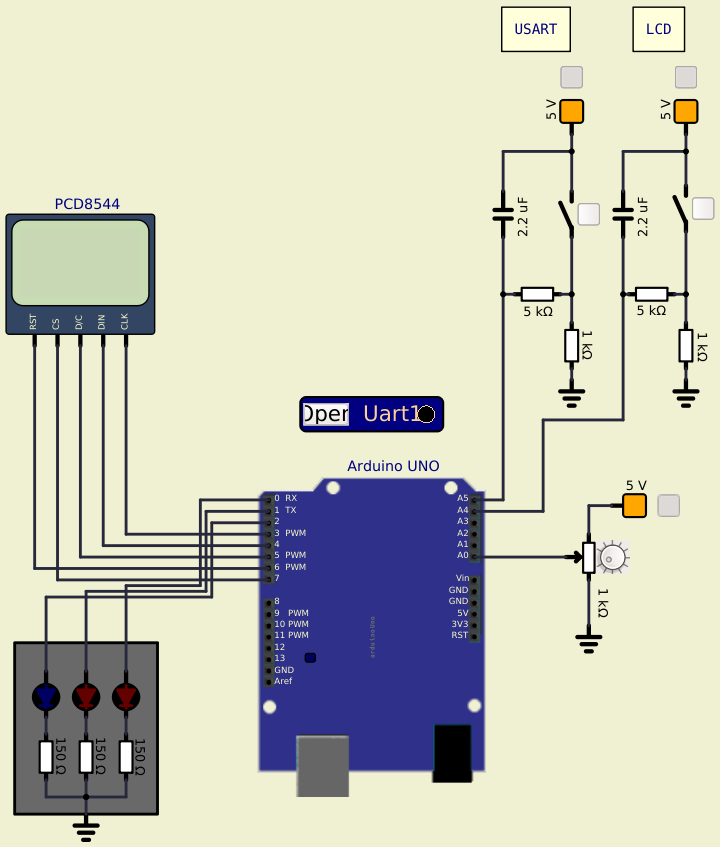
\includegraphics[width=115mm]{./Figuras/Desarrollo_Analisis/final}
\caption{Circuito final tras los cálculos de magnitudes y la implementación de las consideraciones necesarias.} 
\label{fig:final}
\end{figure}

\subsection{Análisis de los resultados}
 A continuación se mostrarán los resultados para cada una de las funcionalidades solicitadas por el enunciado: 

\subsubsection{Temperatura bajo el rango adecuado}
En la Figura \ref{fig:BR} puede observarse el comportamiento de los LEDs en función de la temperatura de salida de la planta cuando esta está por debajo del rango óptimo (30°C $\leq T \leq$ 42°C):

\begin{figure}[H]
\centering
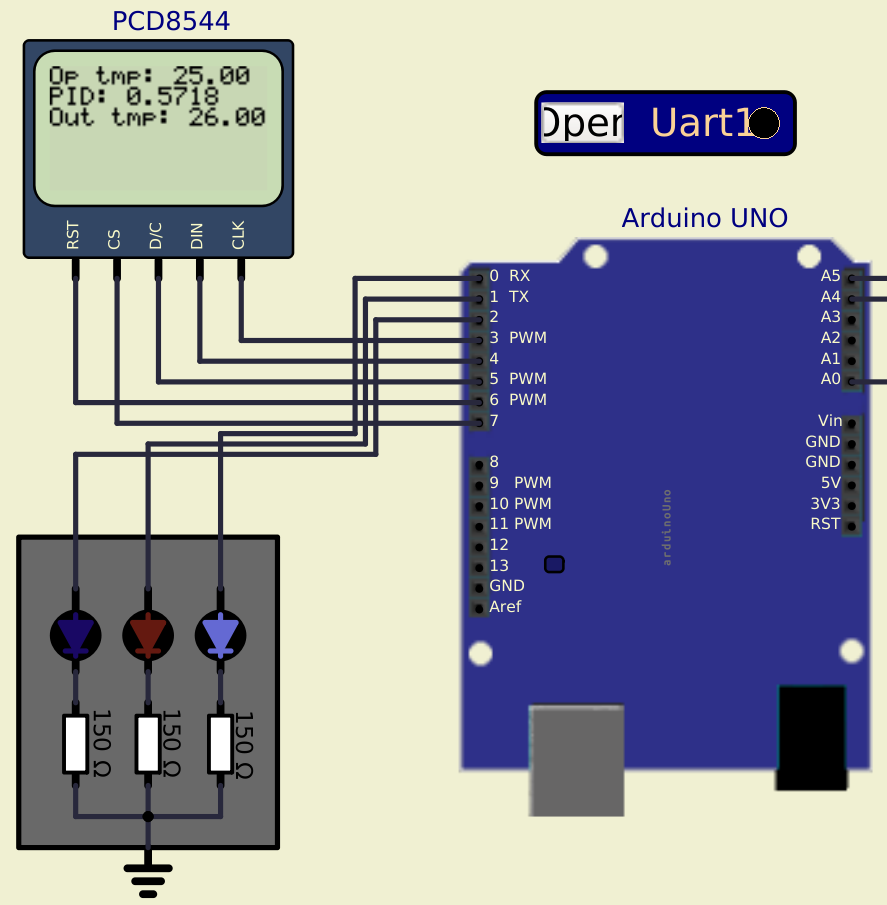
\includegraphics[width=100mm]{./Figuras/Desarrollo_Analisis/BR}
\caption{Funcionamiento del sistema cuando la temperatura de salida de la planta es inferior al rango óptimo de temperatura.} 
\label{fig:BR}
\end{figure}

Como puede verse en la Figura \ref{fig:BR}, el LED azul efectivamente se enciende cuando la temperatura de salida de la planta se encuentra en por debajo del rango óptimo.

\subsubsection{Temperatura dentro del rango adecuado}
En la Figura \ref{fig:DR} puede observarse el comportamiento de los LEDs en función de la temperatura de salida de la planta cuando esta está dentro del rango óptimo (30°C $\leq T \leq$ 42°C):

\begin{figure}[H]
\centering
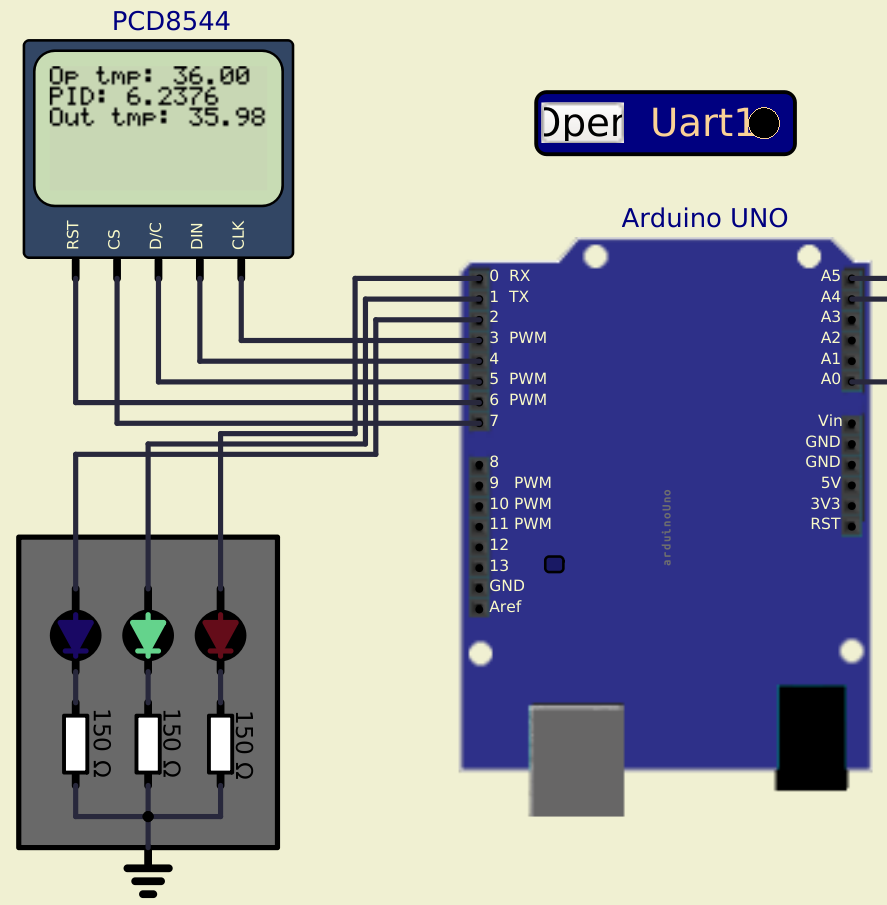
\includegraphics[width=100mm]{./Figuras/Desarrollo_Analisis/DR}
\caption{Funcionamiento del sistema cuando la temperatura de salida de la planta se encuentra dentro al rango óptimo de temperatura.} 
\label{fig:DR}
\end{figure}

Como puede verse en la Figura \ref{fig:DR}, el LED verde efectivamente se enciende cuando la temperatura de salida de la planta se encuentra dentro del rango óptimo.

\subsubsection{Temperatura sobre el rango adecuado}
En la Figura \ref{fig:DR} puede observarse el comportamiento de los LEDs en función de la temperatura de salida de la planta cuando esta está por encima del rango óptimo (30°C $\leq T \leq$ 42°C):

\begin{figure}[H]
\centering
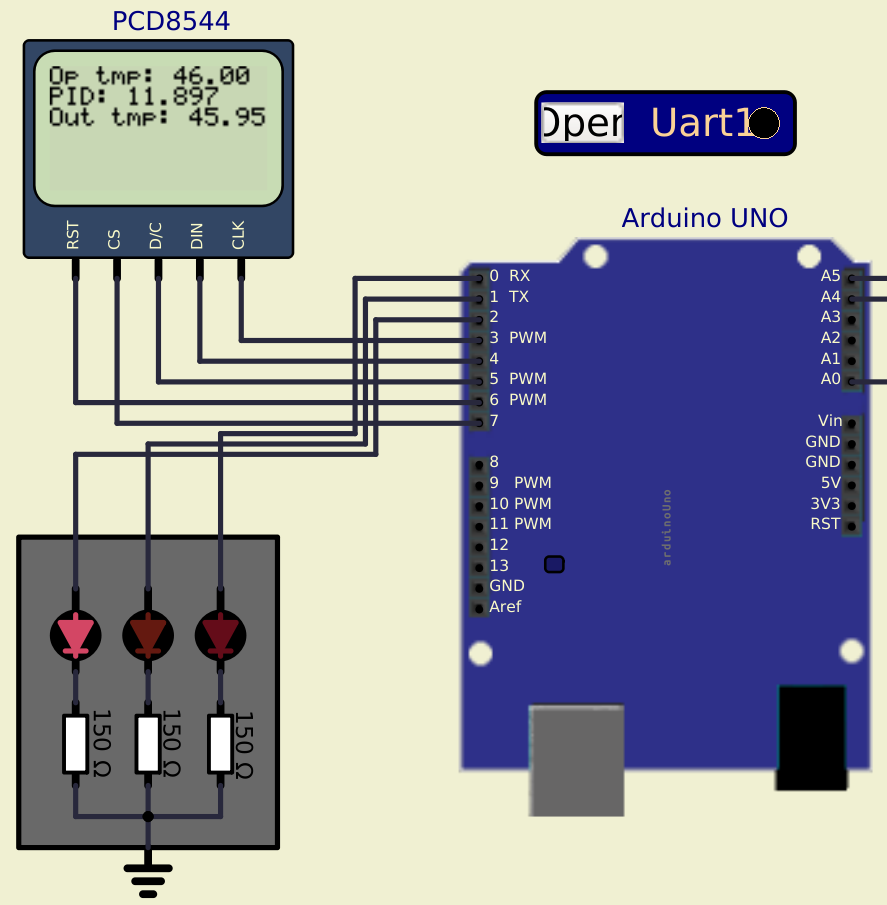
\includegraphics[width=100mm]{./Figuras/Desarrollo_Analisis/SR}
\caption{Funcionamiento del sistema cuando la temperatura de salida de la planta es superior al rango óptimo de temperatura.} 
\label{fig:SR}
\end{figure}

Como puede verse en la Figura \ref{fig:SR}, el LED rojo efectivamente se enciende cuando la temperatura de salida de la planta se encuentra en por encima del rango óptimo.

\subsubsection{Desactivación de la pantalla}
En la Figura \ref{fig:DP} puede observarse el comportamiento del sistema cuando el \textit{switch} que activa la pantalla no fue activado: 

\begin{figure}[H]
\centering
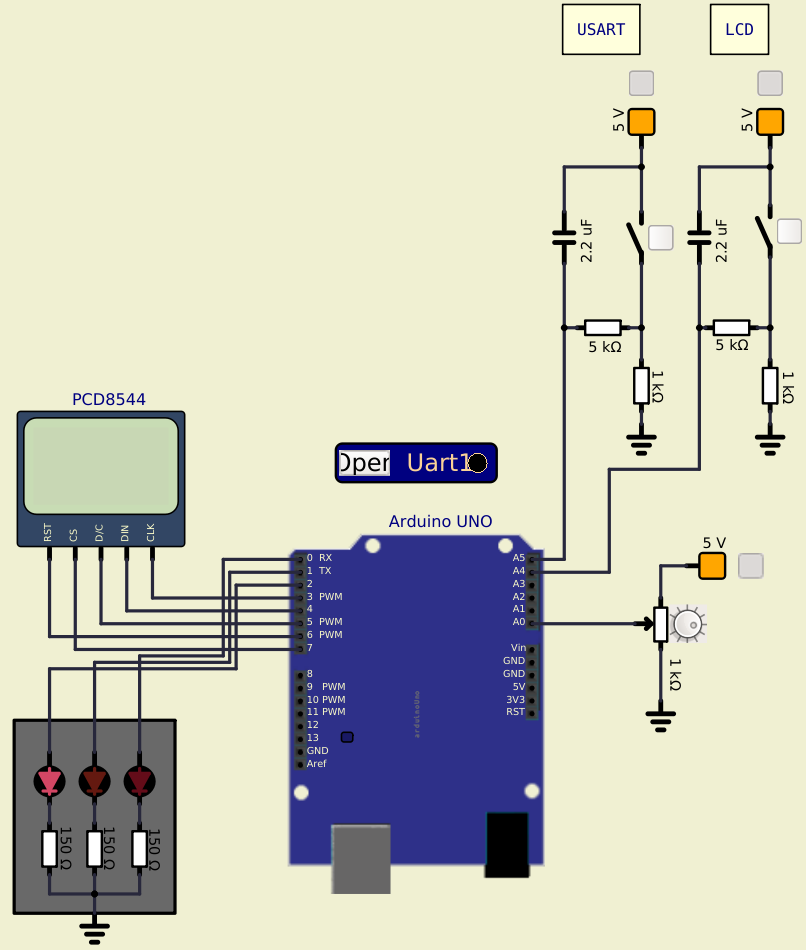
\includegraphics[width=115mm]{./Figuras/Desarrollo_Analisis/DP}
\caption{Funcionamiento de la pantalla LCD cuando el \textit{switch} encargado de gestionarla no fue activado.} 
\label{fig:DP}
\end{figure}

Como puede verse en la Figura \ref{fig:DP}, si el \textit{switch} encargado de gestionar el funcionamiento de la pantalla no ha sido activado, esta no proyecta ninguna información y se mantiene apagada, a pesar de que puede verse que el circuito sigue en funcionamiento, ya que el LED rojo está encendido, indicando que se está trabajando en una temperatura superior al rango óptimo.

\subsubsection{Desactivación de la comunicación serial}
A continuación puede verse el estado de la comunicación serial cuando el \textit{switch} que activa la comunicación serial no fue activado (Figura \ref{fig:DS1}) y el caso contrario (Figura \ref{fig:DS2}): 

\begin{figure}[H]
\centering
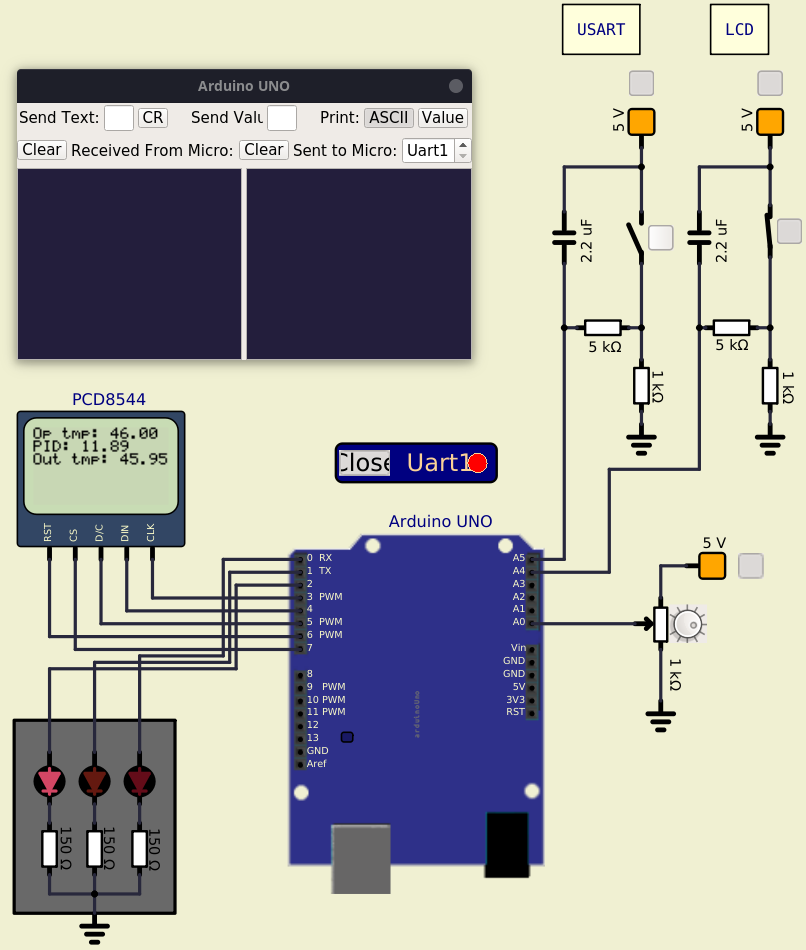
\includegraphics[width=115mm]{./Figuras/Desarrollo_Analisis/DS1}
\caption{Funcionamiento de la salida de datos por el puerto serial cuando el \textit{switch} encargado de gestionarlo no fue activado.} 
\label{fig:DS1}
\end{figure}

\begin{figure}[H]
\centering
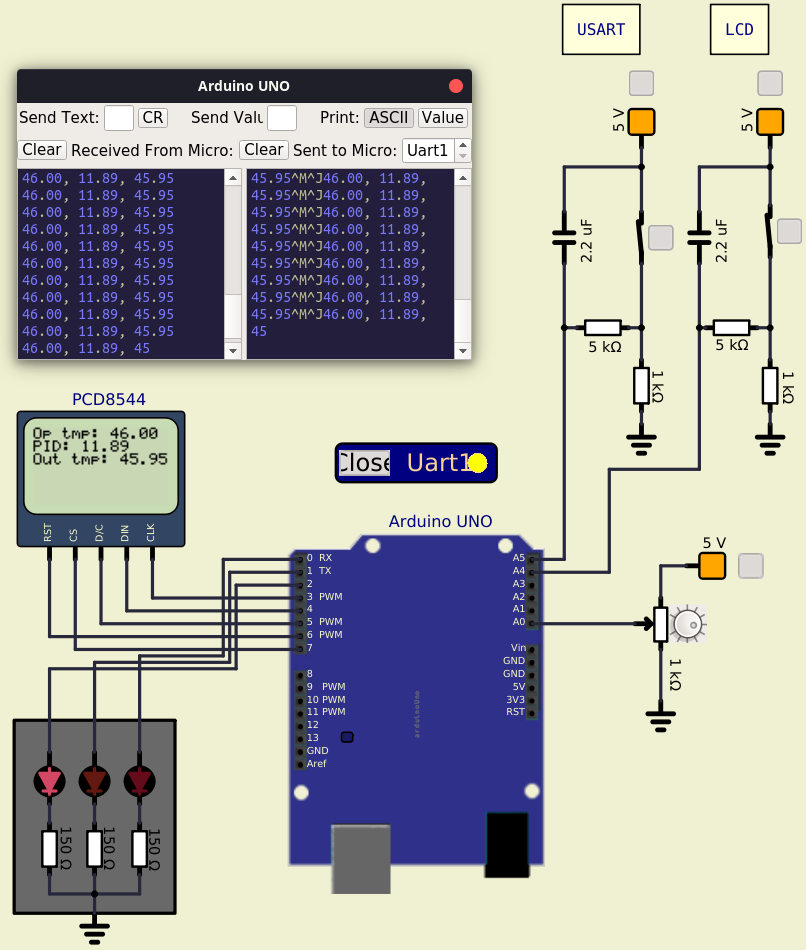
\includegraphics[width=115mm]{./Figuras/Desarrollo_Analisis/DS2}
\caption{Funcionamiento de la salida de datos por el puerto serial cuando el \textit{switch} encargado de gestionarlo fue activado.} 
\label{fig:DS2}
\end{figure}

Como puede verse en las Figuras \ref{fig:DS1} y \ref{fig:DS2}, si el \textit{switch} encargado de gestionar el funcionamiento de la comunicación serial ha sido activado, los datos recopilados por el Arduino son transportados a la computadora a través del puerto virtual y en caso contrario, esto no ocurre. 

\subsubsection{Aumento de temperatura}
A continuación pueden observarse el punto de inicio y final (Figuras \ref{fig:AT1} y \ref{fig:AT2}) y el comportamiento de las señales de temperatura de referencia, señal de control y temperatura de salida antes una disminución en la temperatura (Figura \ref{fig:AT}):

\begin{figure}[H]
\centering
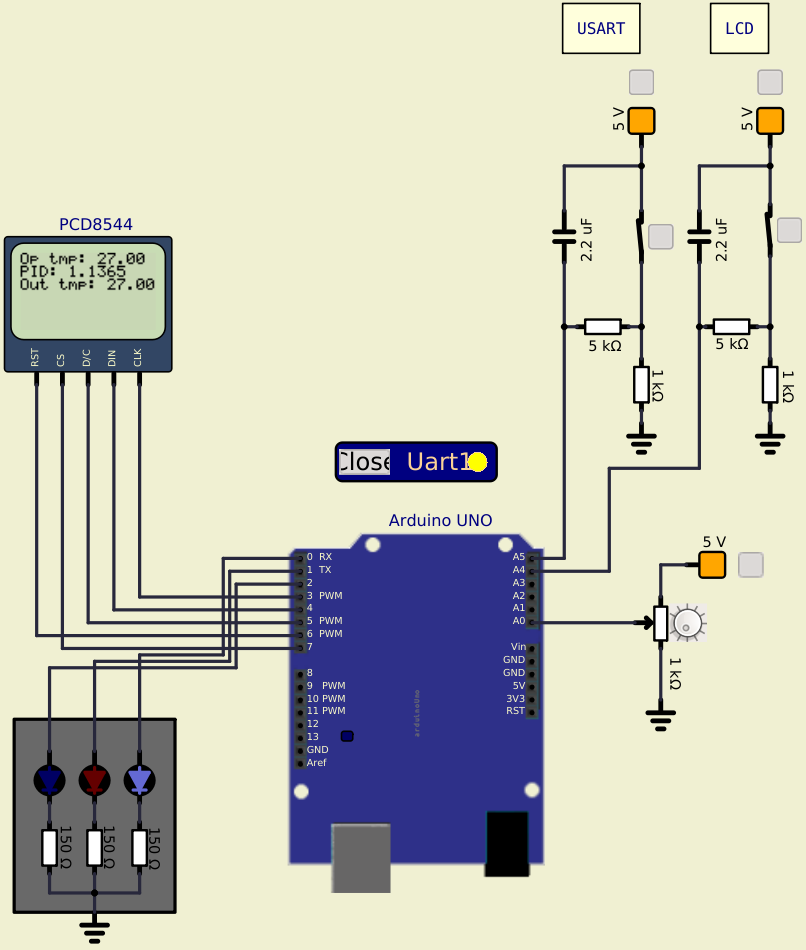
\includegraphics[width=115mm]{./Figuras/Desarrollo_Analisis/AT1}
\caption{Temperatura de inicio antes del aumento.} 
\label{fig:AT1}
\end{figure}

\begin{figure}[H]
\centering
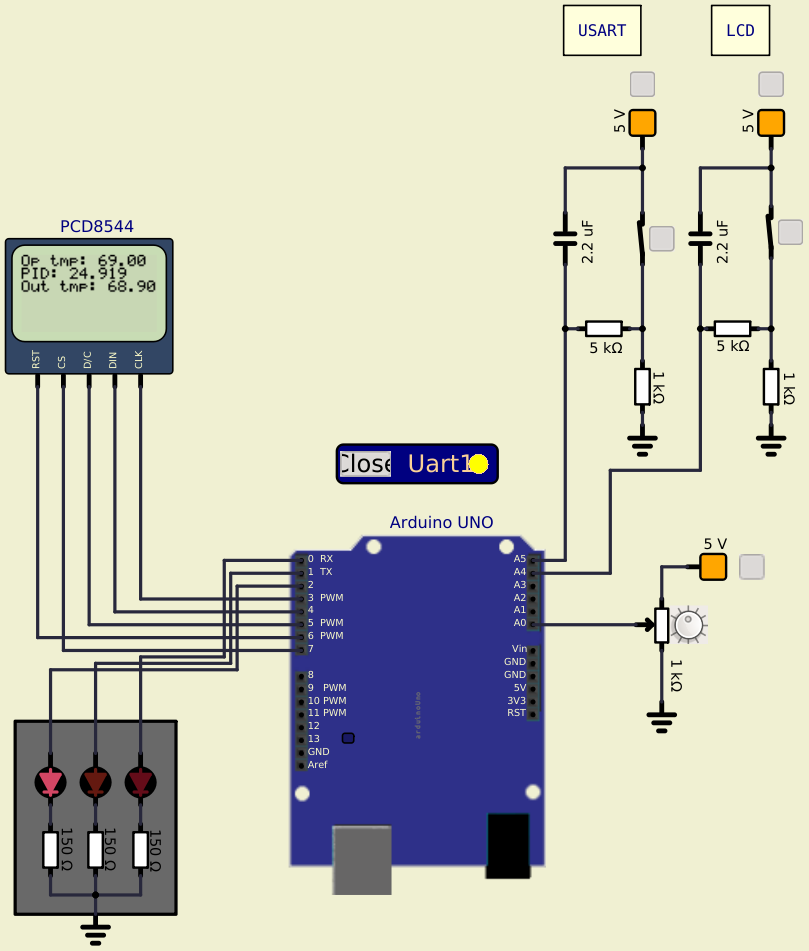
\includegraphics[width=115mm]{./Figuras/Desarrollo_Analisis/AT2}
\caption{Temperatura de final tras el aumento.} 
\label{fig:AT2}
\end{figure}

\begin{figure}[H]
\centering
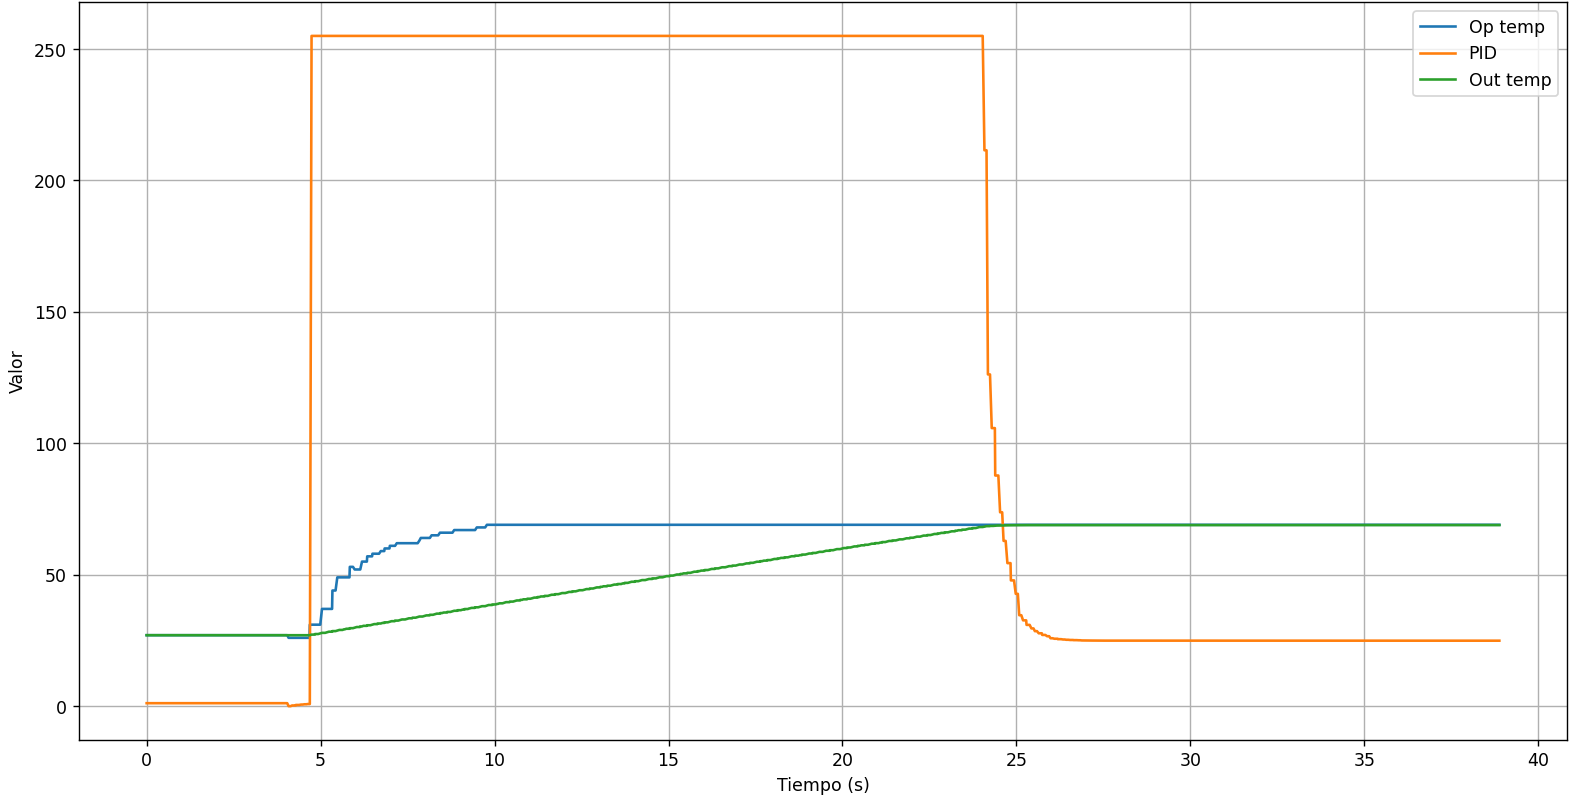
\includegraphics[width=115mm]{./Figuras/Desarrollo_Analisis/AT}
\caption{Gráfica de aumento de temperatura para cada una de las señales de interés.} 
\label{fig:AT}
\end{figure}

Como puede verse en la gráfica de la Figura \ref{fig:AT}, la temperatura de salida sigue rápidamente a la temperatura de referencia, lo cual es un comportamiento esperado (la temperatura debería subir relativamente rápido). Asimismo, se puede ver como la señal de control sube considerablemente para compensar el cambio en la referencia y baja en el momento en el que la señal de salida alcanza el \textit{setpoint}. En la Figura \ref{fig:AT2} puede verse como la temperatura de salida se aproxima casi de manera absoluta a la referencia. 

\subsubsection{Disminución de temperatura}
A continuación pueden observarse el punto de inicio y final (Figuras \ref{fig:DT1} y \ref{fig:DT2}) y el comportamiento de las señales de temperatura de referencia, señal de control y temperatura de salida antes una disminución en la temperatura (Figura \ref{fig:DT}): 

\begin{figure}[H]
\centering
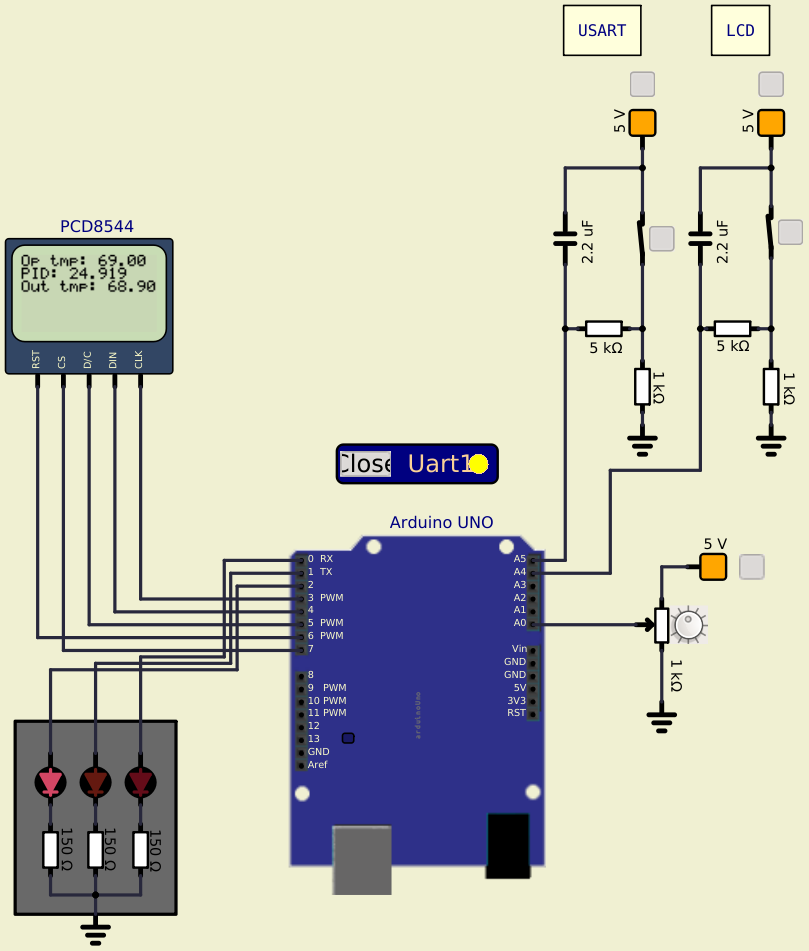
\includegraphics[width=115mm]{./Figuras/Desarrollo_Analisis/AT2}
\caption{Temperatura de inicio antes de la disminución.} 
\label{fig:DT1}
\end{figure}

\begin{figure}[H]
\centering
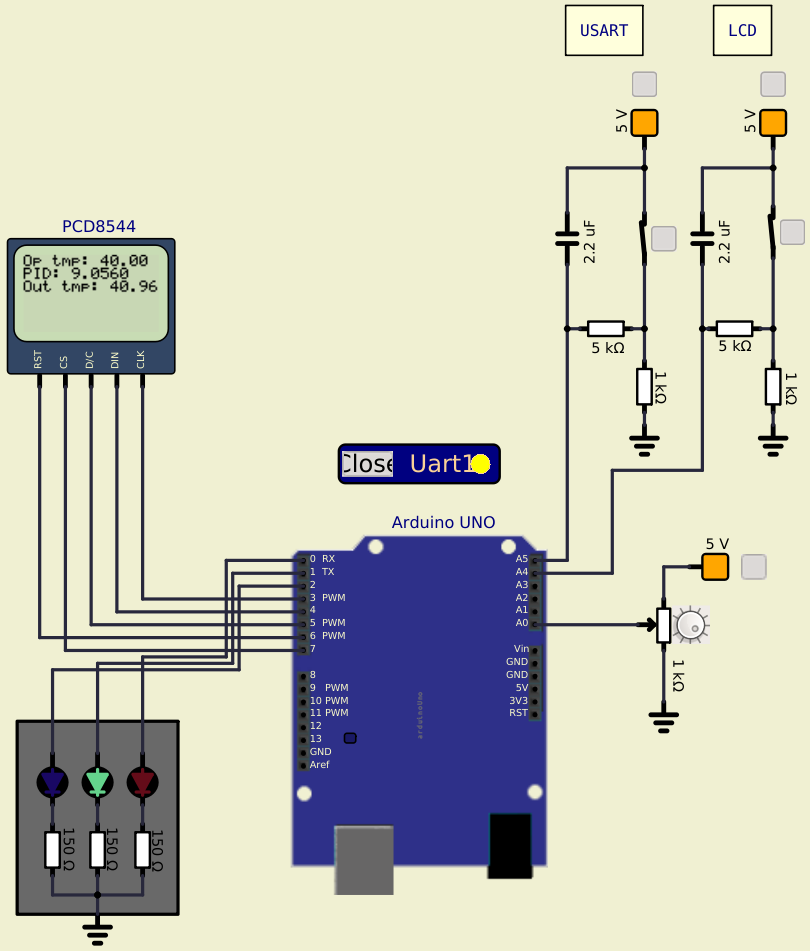
\includegraphics[width=115mm]{./Figuras/Desarrollo_Analisis/DT2}
\caption{Temperatura de final tras la disminución.} 
\label{fig:DT2}
\end{figure}

\begin{figure}[H]
\centering
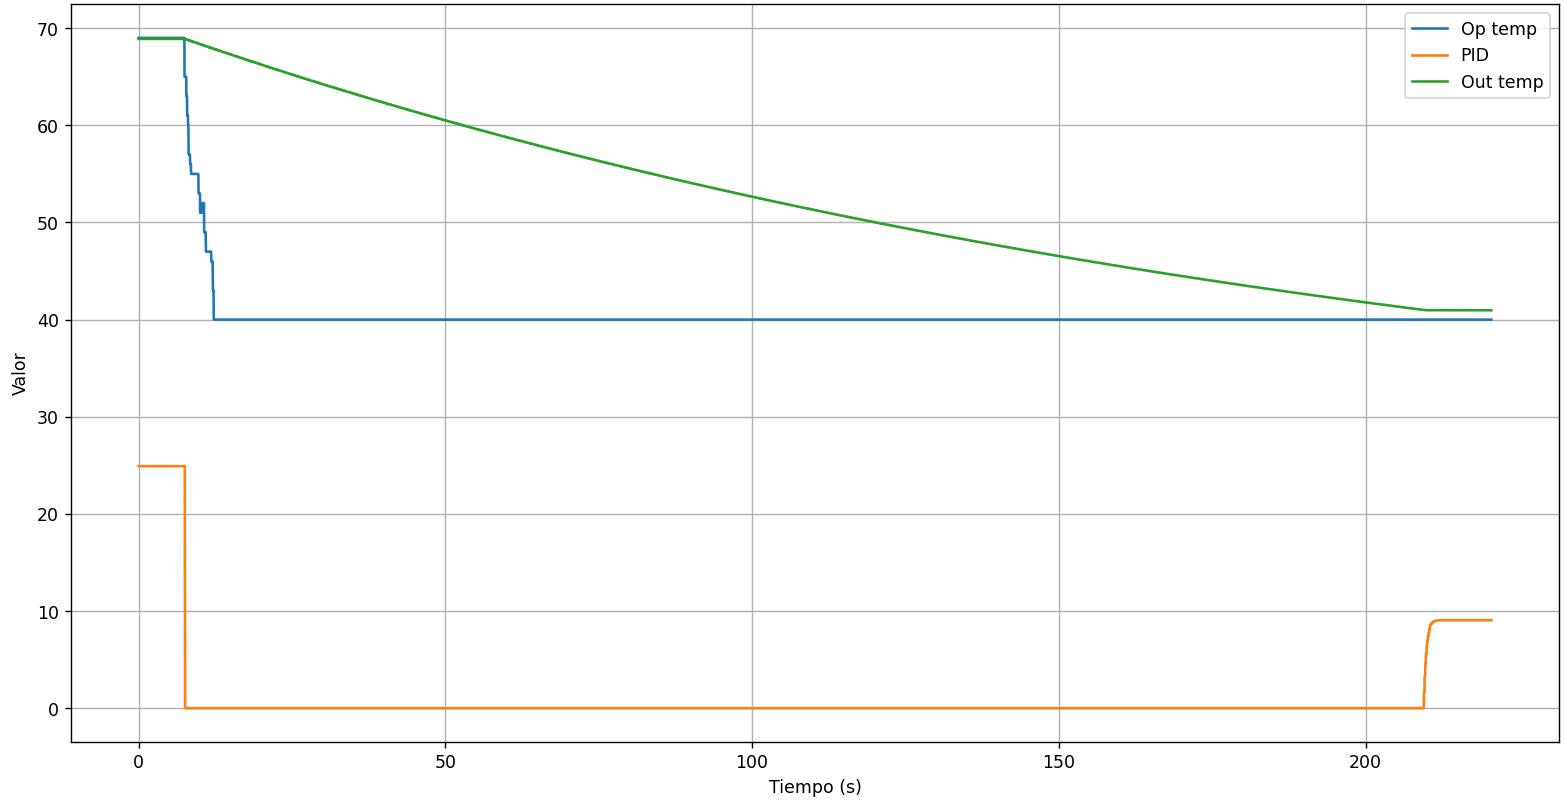
\includegraphics[width=115mm]{./Figuras/Desarrollo_Analisis/DT}
\caption{Gráfica de disminución de temperatura para cada una de las señales de interés.} 
\label{fig:DT}
\end{figure}

Como puede verse en la gráfica de la Figura \ref{fig:AT}, la temperatura de salida sigue lentamente a la temperatura de referencia, lo cual es un comportamiento esperado (la temperatura debería bajar relativamente lento). Asimismo, se puede ver como la señal de control baja para compensar el cambio en la referencia y sube en el momento en el que la señal de salida alcanza el \textit{setpoint}. En la Figura \ref{fig:DT2} puede verse como la temperatura de salida se aproxima casi de manera absoluta a la referencia. 


\newpage
\section{CONCLUSIONES Y RECOMENDACIONES}
A lo largo del desarrollo del informe se pusieron a prueba una serie de conceptos y prácticas importantes para el manejo básico del Arduino UNO, así como sus GPIO, convertidores analógico-digitales, comunicación serial y formas de programación. A continuación algunas conclusiones y recomendaciones recolectadas a lo largo de trabajo realizado: 

\begin{itemize}
    \item Se confirma que el sistema responde correctamente a diferentes rangos de temperatura, como se evidencia en la activación de los LEDs correspondientes dependiendo de si la temperatura está por debajo, dentro o por encima del rango óptimo. Esto indica una adecuada detección y respuesta del sistema a las condiciones térmicas requeridas.

    \item  Se observa que la desactivación de la pantalla y la comunicación serial ocurren como se espera cuando los respectivos \textit{switches} no son activados. Esto sugiere un buen funcionamiento de las funciones adicionales de control y comunicación, lo cual es esencial para el funcionamiento global del sistema.

    \item Los resultados de aumento y disminución de temperatura muestran una respuesta coherente del sistema, donde la señal de control se ajusta apropiadamente para mantener la temperatura de salida cerca de la temperatura de referencia. Esto indica una efectiva regulación térmica y una capacidad de respuesta dinámica del sistema.

    \item Es recomendable realizar pruebas adicionales en condiciones extremas o inesperadas para evaluar la robustez del sistema. Esto ayudaría a identificar posibles vulnerabilidades o escenarios no contemplados durante el diseño inicial.

    \item Dado el buen funcionamiento general del sistema, sería beneficioso agregar alarmas o notificaciones para alertar a los usuarios en caso de que la temperatura se salga del rango óptimo durante un tiempo prudencial. Esto es especialmente crítico en el caso de una incubadora, donde desviaciones de temperatura podrían dañar los huevos en desarrollo.
\end{itemize} 

\newpage
\section*{REFERENCIAS BIBLIOGRÁFICAS} 
\renewcommand*{\refname}{\vspace*{-2em}} 
\bibliographystyle{ieeetr}
\bibliography{bibliografia.bib}

\newpage
\section{Anexos}


\subsection{Hoja del fabricante del ATmega328P Atmel: información general} \label{an:01_GEN}
\vspace{\fill}
\includepdf[pages={1-7}]{./Documentos/Atmel-7810-ATmega328P_Datasheet.pdf} 


\end{document}